\documentclass[../thesis.tex]{subfiles}
% Separate preamble for this subfile. This preamble is loaded last, so one can override various functions before \begin{document}

% Better comment extension for Vscode colors these comments differently
% Normal comment color
% * Important information
% ! ALERT
% ? Question
% TODO stuff to do
% // This is strikethrough


\begin{document}
Informally, to tile refers to the process of covering some surface with objects. These objects are called tiles and come in a variety of shapes and sizes. When we are tiling, we essentially place copies of the tile next to each other in a systematic way, intending to leave no gaps and no overlaps between the tiles \cite{kolountzakisTilingsTranslation2010}. The resulting tiling can be as simple as the one shown in \cref{fig:tiling_one} where we have used a single tile, the unit square, to tile the plane, or as complex as \cref{fig:tiling_two} where we have used four different tiles to tile the plane. The first is an example of what is known as a \emph{monohedral tiling} in which all tiles are congruent, and the latter is an example of a Penrose tiling which are well known for being non-periodic \cite[p. 20, 531]{grunbaumTilingsPatterns1987}. %* 1979 page 535 har også penrose tilings

%! Figure input here



\begin{figure}[h!]%h!
    \centering
    \begin{subfigure}{.47\textwidth}
        \centering
        %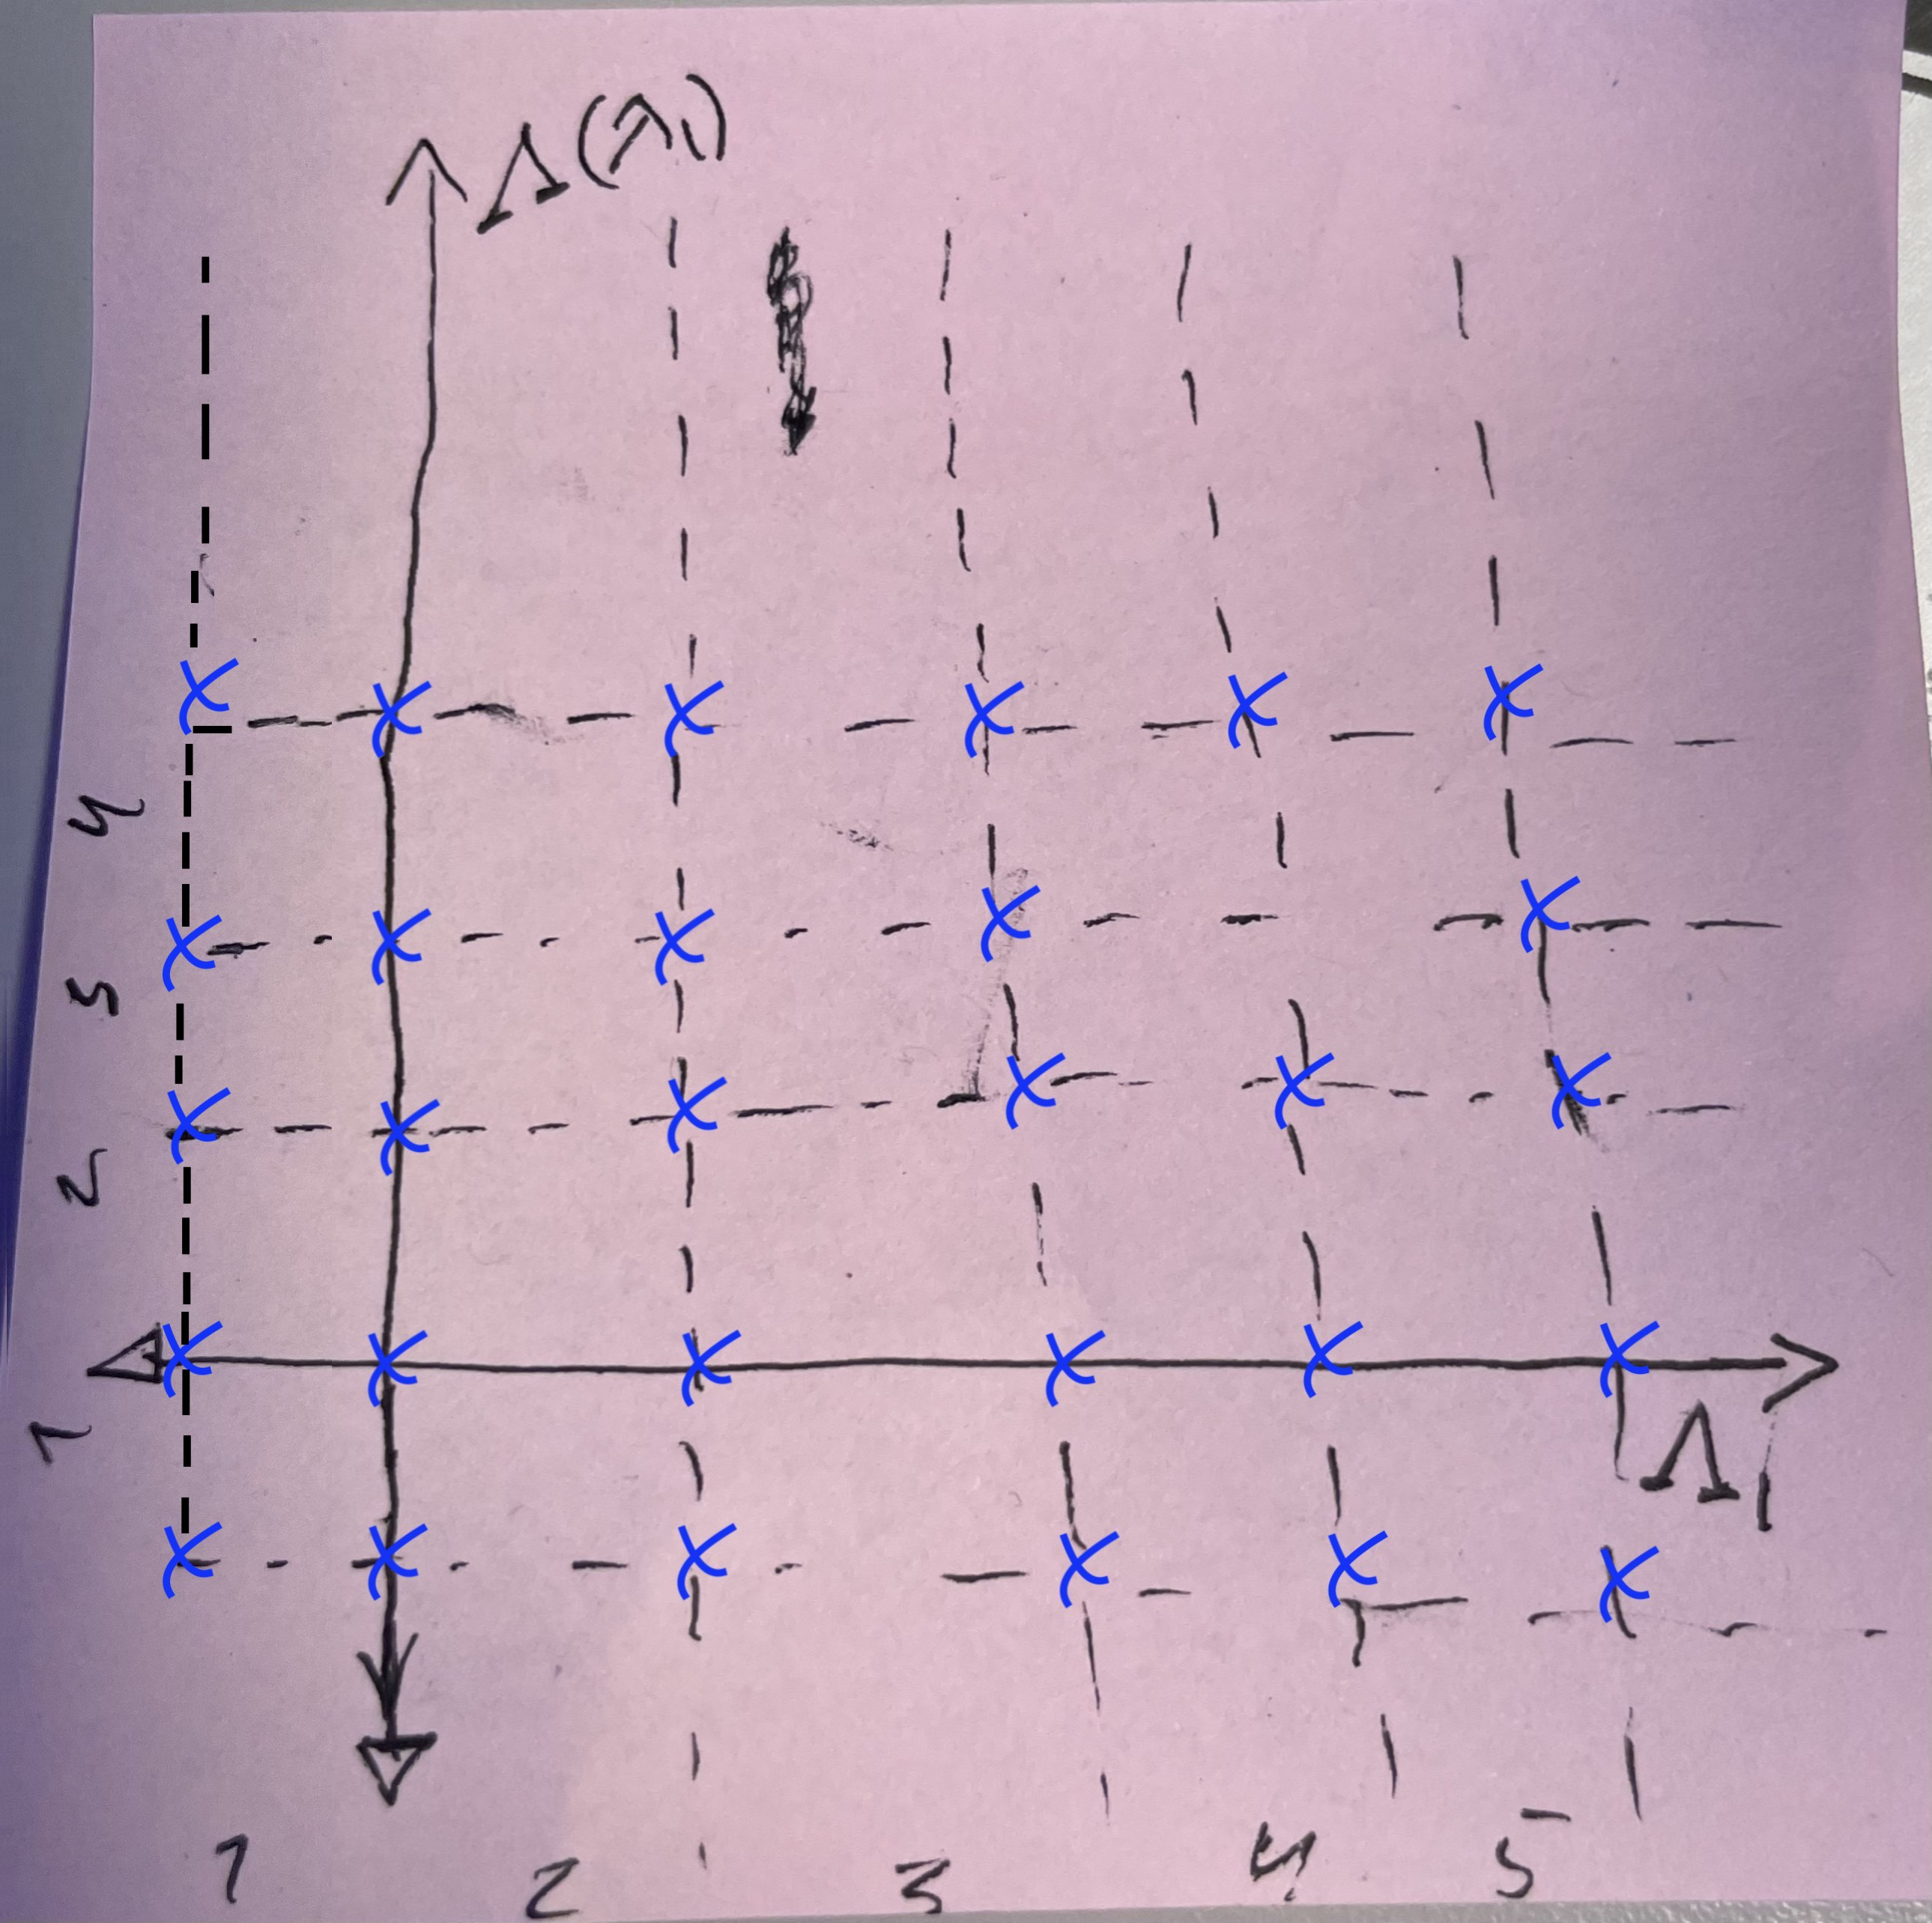
\includegraphics[width=0.9\linewidth]{spec_no_shift.jpg}
        %* Figure 1
        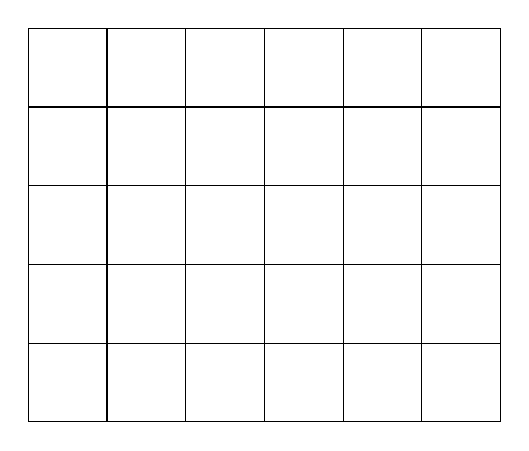
\begin{tikzpicture}[scale=1]
            % Define the tile
            \def\tile{
              % Draw the unit square
              \draw (0,0) rectangle (1,1);
            }
          
            % Draw the tiling pattern
            \foreach \x in {0,1,2,3,4,5}{
              \foreach \y in {0,1,2,3,4}{
                \pgfmathsetmacro{\shiftX}{\x} % Set horizontal shift
                \pgfmathsetmacro{\shiftY}{\y} % Set vertical shift
                \begin{scope}[shift={(\shiftX,\shiftY)}]
                  \tile % Draw the tile
                \end{scope}
              }
            }
        \end{tikzpicture}
        %* —————————————————
        \caption{Lattice tiling}
        \label{fig:tiling_one}
    \end{subfigure}\quad
    \begin{subfigure}{.47\textwidth}
        \centering
        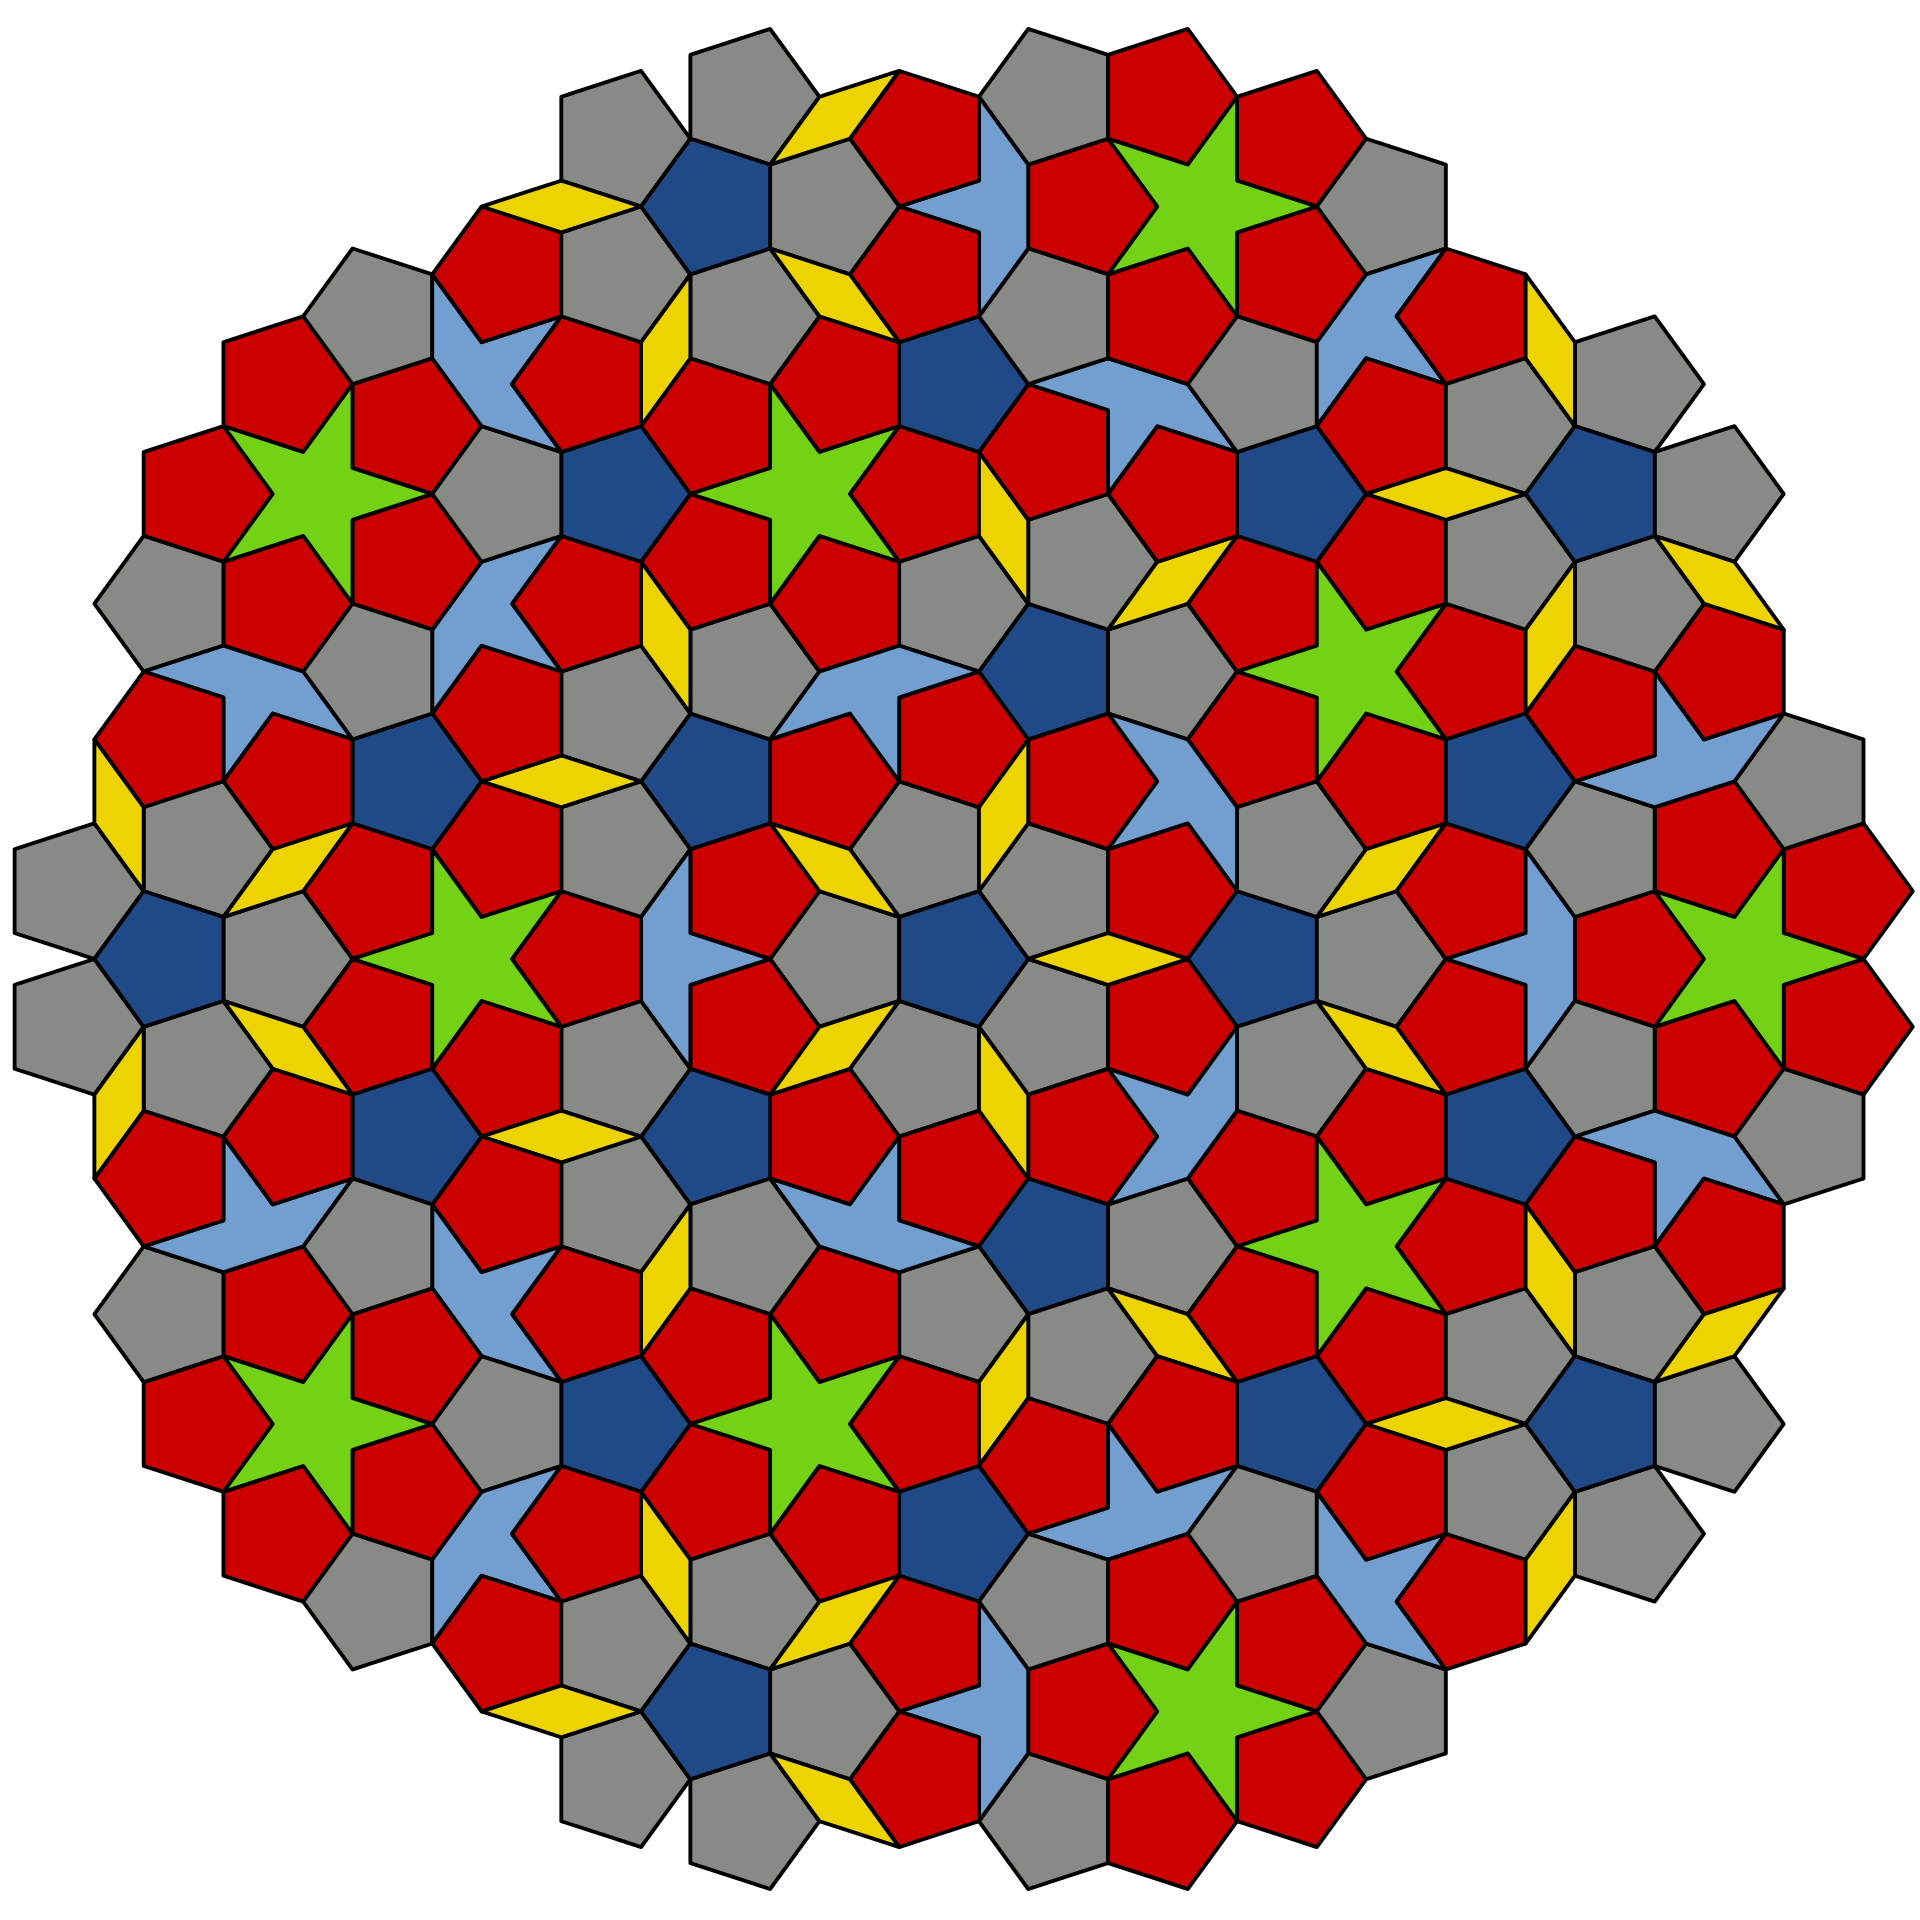
\includegraphics[width=0.87\linewidth]{Penrose_Tiling_.png}
        \caption{P1 Penrose tiling \cite{inductiveloadP1TilingUsing}}
        \label{fig:tiling_two}
    \end{subfigure}
    \caption{Two contrasting tilings of the plane to emphasize the range of complexity. \cref{fig:tiling_one} shows a simple monohedral tiling, and \labelcref{fig:tiling_two} shows an intricate, non-periodic tiling using four different tiles. The coloring in the latter is used to distinguish the tiles more easily and highlight the three \emph{matching rules} for the pentagonal tiles, the only ones with different colors for the same shape. Matching rules are needed in order to tile aperiodically \cite{penrosePentaplexityClassNonPeriodic1979}.}
    \label{fig:tilings_one_two}
\end{figure}

% Penrose goes into the details of these in his paper 

\mycomment{  %! Block comment
The lattice tiling in \labelcref{fig:tiling_one} has fewer tiles and lacks variety compared to Penrose's original aperiodic tiling.

Two tilings of the plane to emphasize the contrast between monohedral tilings and an intricate tiling
Two tilings of the plane emphasize the contrast from monohedral tilings to more intricate tilings, such as the Penrose tiling in Fig. 

Two contrasting tilings of the plane between a monohedral tiling in \cref{fig:tiling_one} and more intricate tilings such as the Penrose tiling in \cref{fig:tiling_two} 

In contrast to the simple monohedral tiling shown in \cref{fig:tiling_one}, the Penrose tiling in \cref{fig:tiling_two} and other intricate tilings provide contrasting examples of tilings on the plane.
In contrast to the simple monohedral tiling shown in \cref{fig:tiling_one}, the Penrose tiling in \cref{fig:tiling_two} is a contrasting example of a more intricate tiling of the plane. 
In contrast to the simple monohedral tiling shown in \cref{fig:tiling_one}, the Penrose tiling in \cref{fig:tiling_two} is an example of a more intricate tiling of the plane. 

Two contrasting tilings of the plane to emphasize the stark difference between a simple monohedral tiling in \cref{fig:tiling_one} and more intricate tilings such as the Penrose tiling in \cref{fig:tiling_two}.
Two contrasting tilings of the plane to emphasize the stark difference between a simple monohedral tiling in \cref{fig:tiling_one} and a more intricate tiling in \cref{fig:tiling_two} which is non-periodic and uses four tiles. 

To emphasize the stark difference between a simple monohedral tiling in \cref{fig:tiling_one} and a more intricate tiling in \cref{fig:tiling_two} which is non-periodic and uses four tiles, we present two contrasting tilings of the plane.

Two contrasting tilings of the plane to emphasize the range of complexity. \cref{fig:tiling_one} shows a simple monohedral tiling, and \cref{fig:tiling_two} shows an intricate, non-periodic tiling using four different tiles. 
} 

Another interesting pair of monohedral tilings is given in \cref{fig:tiling_three,fig:tiling_four}. These are both examples of an Escher tiling in which a lizard and horseman tile the plane. Note that in comparison to the square tilings in \cref{fig:tiling_one}, there is important to highlight two fundamental differences between the square and Escher tilings. The first is that one needs to rotate the lizard to cover the entire surface, and the second is that one needs to reflect the horseman to cover the entire surface. It is these three motions and combinations of them that we use when tiling in general \cite[p. 26]{kolountzakisTilingsTranslation2010,grunbaumTilingsPatterns1987}. 

%! Figure input here



\begin{figure}[t]%h!
    \centering
    \begin{subfigure}{.47\textwidth}
        \centering
        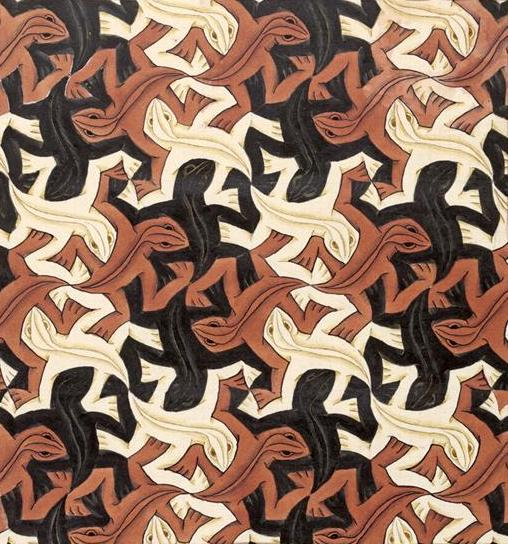
\includegraphics[width=0.9\linewidth]{lizard-1.jpg}
        \caption{Lizard}
        \label{fig:tiling_three}
    \end{subfigure}\quad
    \begin{subfigure}{.47\textwidth}
        \centering
        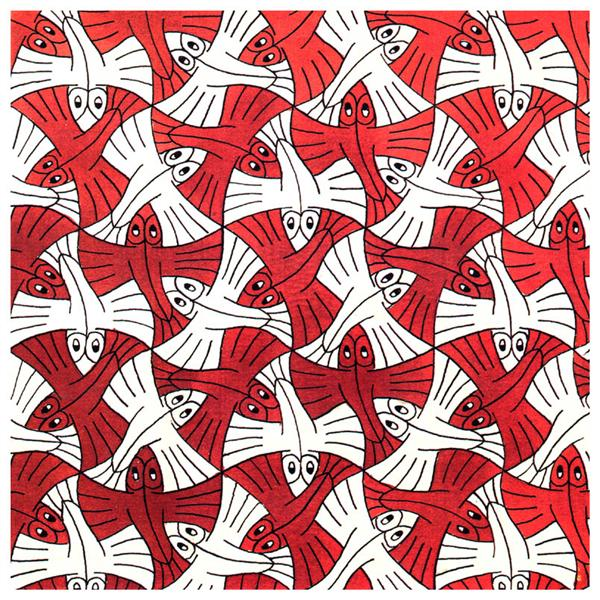
\includegraphics[width=0.9\linewidth]{flying-fish.jpg}
        \caption{Flying fish}
        \label{fig:tiling_four}
    \end{subfigure}
    \caption{Text}
    \label{fig:tilingsss_two}
\end{figure}

\section{Cube-tilings: Keller's Theorem and Keller's Conjecture}
    \subfile{03_x1__cube_gen}


\section{Exotic tilings; Non-periodic tilings}
    \subfile{03_x2__non-periodic}

\section{Exotic tilings; Aperiodic tilings}\label{sec:aperi_cube}
    \subfile{03_x3__aperiodic}

\section{Proof of Keller's Theorem}\label{sec:proof_keller}
    \subfile{03_x4__proof_keller}

%* Ikke si så veldig mye, 
%* Når vi kommer opp i d=2, så har vi åpenbart mer fleksibilitet, selv om Kellers theorem fortsatt er sant. Sånn at vi har jo den begrensningen om at vi må møtes i et heltall. 
%* Vise flexen og referere til kellers - Nei — Ikke begrunne det med Keller, 
%* I to dimensjoner har vi åpenbart større fleksibilitet fordi vi ikke trenger å ha Lattice tiling. Det kan vi vise ved eksempel. Dette ser vi i figur sånn og sånn, men det som også kommer frem så oppfyller jo Alle Kellers theorem, og det vil de også måtte gjøre. Det ville jeg kommentert, uten å, liksom, begrunne det til noe som helst.
%* Dette for å si noe om det (fleksibiliteten vi skal fange) allerede her
%* Vi skal se senere, (kap 5), det vi har tegnet her, strenkt tatt fanger all den fleksibiliteten vi har. Du har ikke noe mer fleksibilitet enn det du har skissert her. Du kan skyve på kolonnene, og du kan skyve på radene. Men det kommer vi tilbake til den og den seksjonen. Prøvd å skiserre. Da viser den figuren her egentlig all den fleksibiliteten vi har, men ikke sagt at du skal skal forklare noe mer om det nå. 
\end{document}


